% THIS IS SIGPROC-SP.TEX - VERSION 3.1
\documentclass{sig-alternate}

% Additional packages
\usepackage{graphicx}
\usepackage{color}
\usepackage{url}
\usepackage{algorithm}
\usepackage[noend]{algpseudocode}
\usepackage{amsmath}
%\usepackage{amsthm}
\usepackage{amsfonts}
\usepackage{amssymb}
\usepackage{booktabs}
\usepackage{multirow}
\usepackage{ifpdf}
% Custom commands
%\usepackage{custom_commands}

%\newcommand{\note}[1]{\relax} %{\color{red}#1}}
\newcommand{\note}[1]{{\color{red}#1}}

\newcommand{\prg}[1]{\paragraph{#1}}
%\newcommand{\prg}[1]{\textbf{#1}}

\newcommand{\Siren}{\textsc{Siren}}
\newcommand{\ReReMi}{\textsc{ReReMi}}

\begin{document}
\special{papersize=8.5in,11in}
\setlength{\pdfpageheight}{11in}%{\paperheight}
\setlength{\pdfpagewidth}{8.5in}%{\paperwidth}


\title{Siren: An Interactive Tool for Mining Geospatial Redescriptions}
\subtitle{[Demo]}

\numberofauthors{2} 
\author{
% 1st. author
\alignauthor
Esther Galbrun\\
       \affaddr{Department of Computer Science}\\
       \affaddr{University of Helsinki, Finland}\\
       \email{galbrun@cs.helsinki.fi}
% 2nd. author
\alignauthor
Pauli Miettinen\\
       \affaddr{Max Plack Institute for Informatics}\\
       \affaddr{Saarbr{\"u}cken, Germany}\\
       \email{pmiettin@mpi-inf.mpg.de}
}

\maketitle
\begin{abstract}
  We present \Siren, an interactive tool for mining geospatial
  redescriptions.  Redescription mining is a powerful data analysis
  tool that aims at finding alternative descriptions the same
  entities.  For example, in biology, an important task is to identify
  the bioclimatic constraints that allow some species to survive, that
  is, to describe geographical regions in terms of both their
  bioclimatic conditions and the fauna that inhabits them.  When the
  entities are geographic locations, we qualify the redescriptions as
  geospatial.  Using \Siren, a user can explore data of his
  interest by visualizing geospatial redescriptions on a map,
  interactively edit, extend and filter them\footnote{More details about \Siren's features and a demonstration video are available online at \url{http://www.cs.helsinki.fi/u/galbrun/redescriptors/siren/}.}. 
  We will demonstrate our
  system on two data sets, one about European mammals and climate, the
  other containing US census and election funding data.
\end{abstract}

\category{H.2.8}{Information Systems}{Database Applications}[Data Mining]
\category{H.5.2}{Information Interfaces and Presentation}{User Interfaces}

\terms{Redescription Mining, Geospatial data, Application}

%\keywords{ACM proceedings, \LaTeX, text tagging} % NOT required for Proceedings

\section{Introduction}
%\subsubsection{Redescription Mining}
Finding multiple ways to characterize the same entities is an
important way of gaining insight in your data.  In \emph{Redescription
Mining}, the input contains entities with two sets of characterizing
variables. The task is to find a pair of queries, one query for both
sets of variables, such that both queries describe (almost) the same
set of entities.

%\note{Two views of redescription mining}
The results of redescription mining, the redescriptions, can be
approached from two points of view. On one hand, we can study the
variables and conditions appearing in the redescriptions, giving us
valuable information about these variables. On the other hand, we can
study the support set of the redescriptions, i.e.\ the set of
observations where both queries of a redescription hold. When the data
is geospatial, that is, the observations are connected to locations, the
latter approach becomes even more important. A meaningful geospatial
redescription should define coherent areas using expressive
queries. The goal of \Siren\ is to facilitate the analysis of the
redescriptions using both of the approaches simultaneously.

\begin{figure}[hb]
  \centering
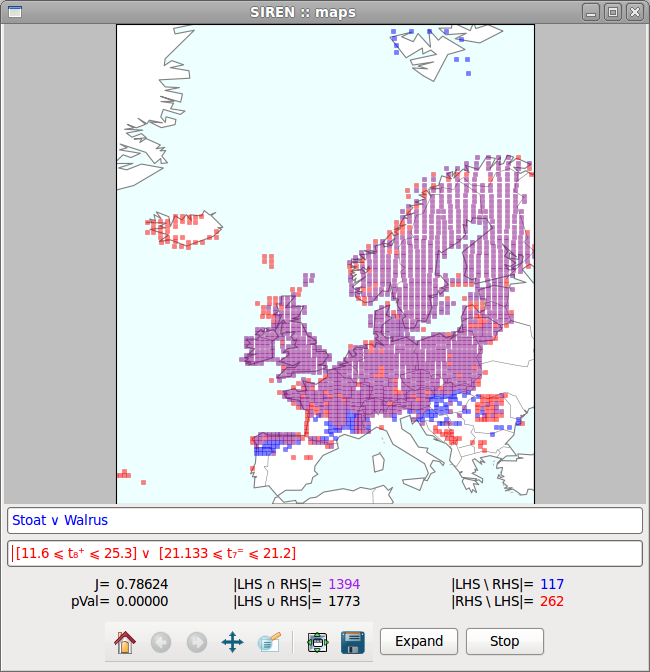
\includegraphics[width=.5\textwidth]{screenshots/siren_map.png}
  \caption{Map panel, displaying a redescription on a map.}
  \label{fig:map_panel}
\end{figure}

\begin{figure*}[t]
  \centering
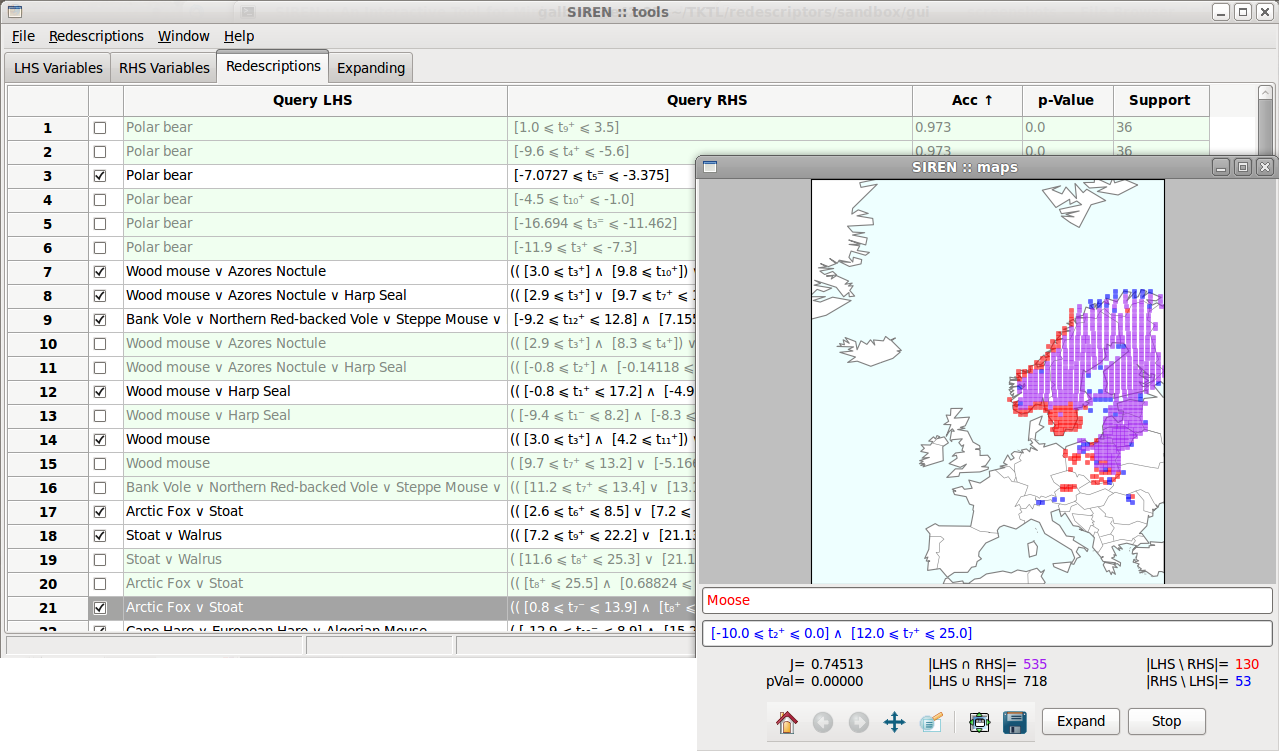
\includegraphics[width=\textwidth]{screenshots/both_panels_02.png}
  \caption{Siren}
  \label{fig:both_panels}
\end{figure*}


\section{Use-case scenario}
\label{sec:scenarios}
We exemplify the use \Siren\ by going through a typical workflow
of mining geospatial redescriptions.

\prg{Initial redescription mining}
Given the data, a natural first step is to use a redescription mining
algorithm to find the initial set of redescriptions. \Siren\ relies the
\ReReMi\ algorithm~\cite{galbrun11black} for this. 

When the initial set of redescriptions is mined, the user can study the
interesting redescriptions plotted on a map (see
Fig.~\ref{fig:map_panel}).
Uninteresting redescriptions can be manually disactivated.

 
\prg{Editing a redescription} 
The true strength of \Siren\ comes to play after the initial set of
redescriptions is mined, as it allows the user to visualize, edit,
filter and refine the redescriptions.  It is typical that the
algorithm returns redescriptions that the user wants to edit. For
example, some redescriptions might be overly complex, or have
exceedingly accurate boundaries for numerical variables. The user can
easily select the redescription he wants to modify, open it in a map
window and start editing it. \Siren\ updates the map and important
statistics (accuracy, $p$-value, etc.) about the redescription,
allowing the user to see the effects of his edits immediately. This
makes it easy for the user to check, e.g.\ whether the simplified
redescription would still be acceptably accurate.


\prg{Extending a redescription}
Sometimes the user wants to focus only on one of the queries in the
redescription, on some particular variable of interest or on part of an existing redescription. 
\Siren\ allows the user to automatically extend a given
redescription, i.e.\ let the algorithm add new items to the queries to
make the redescription as accurate as possible (see
Fig.~\ref{fig:extending}). 

The extension mechanism of \Siren\ uses the beam search implemented in
the \ReReMi\ algorithm.  It can also be used to explore more specific
alternative extensions to a redescription, that the beam search might
have discarded at some point of the search because they were not the
best extensions.


\begin{figure*}
  \centering
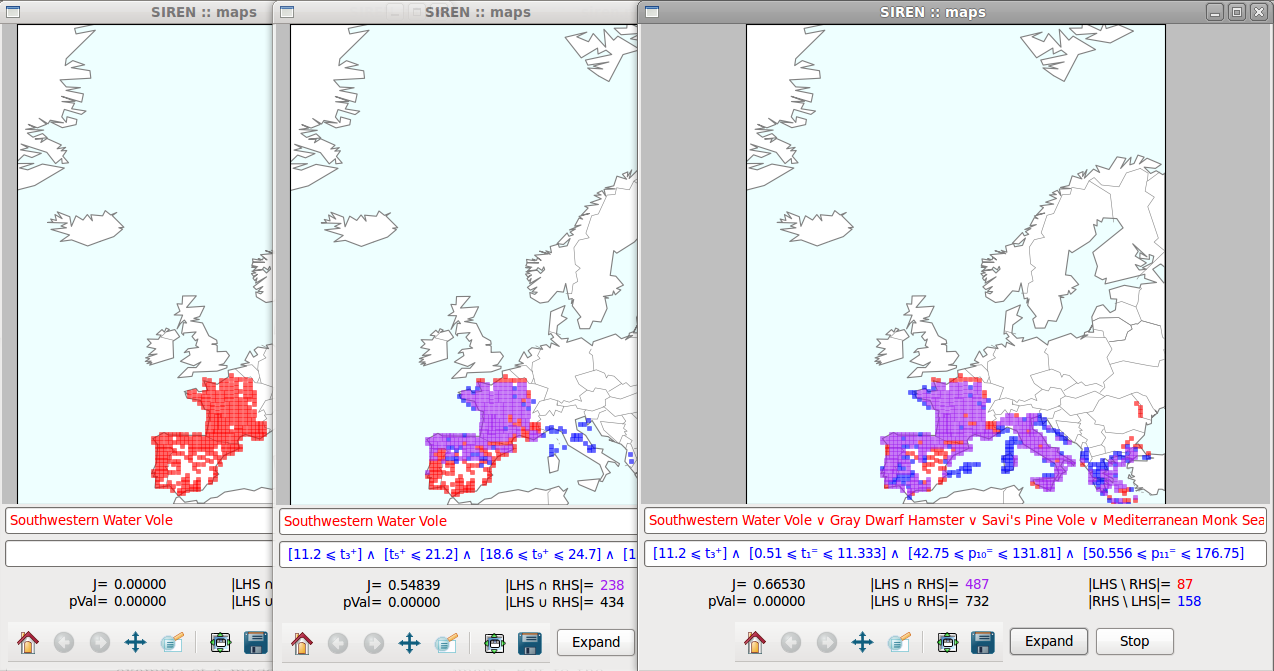
\includegraphics[width=\textwidth]{screenshots/comparison.png}
  \caption{Map panels, comparing redescriptions.}
  \label{fig:comparison}
\end{figure*}



\prg{Using subsets of variables}
Finally, many times a set of redescriptions contain the same pair of
variables. This can happen, e.g.\ when these two variables are highly
correlated. The user, however, might want to see redescriptions that have
only one of these variables, not both. \Siren\ makes this simple: the user
only has to select a redescription, remove the variable he does not
want to have from the redescription, unselect it from the list of variables, and
extend the redescription. \Siren\ will not use the unselected
variables when extending or mining redescriptions.


\begin{figure}
  \centering
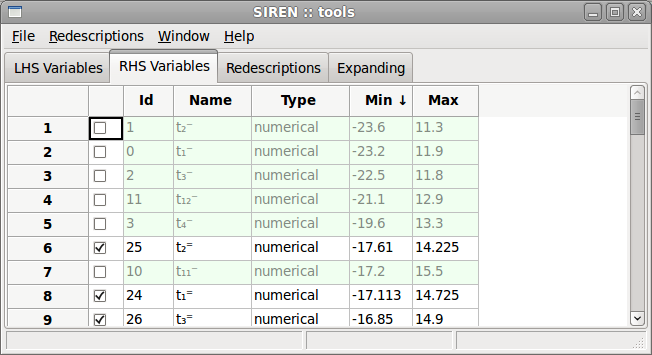
\includegraphics[width=.5\textwidth]{screenshots/variables_05.png}
  \caption{Tool panel, uselecting variables.}
  \label{fig:map_panel}
\end{figure}

\begin{figure}
  \centering
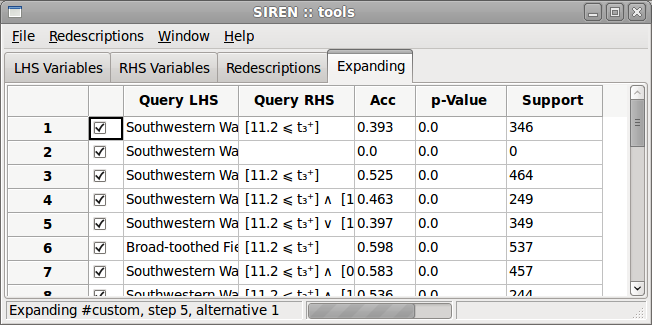
\includegraphics[width=0.5\textwidth]{screenshots/extending.png}
  \caption{Tool panel, extending a redescription.}
  \label{fig:extending}
\end{figure}



\prg{Filtering redundant redescriptions}
\label{sec:filt-redund-redescr}
It is common to see a set of redescriptions that cover approximately
the same area even if they have (somewhat) different set of
variables. In such cases it is important to be able to recognise and
remove redundant redescriptions, i.e.\ redescriptions that do not
convey significant new information, lest the user be overwhelmed with
the number of found redescriptions. Again, \Siren\ allows automatic
filtering of redundant redescriptions. The user can either select a
redescription and ask \Siren\ to filter out all redescriptions that
are redundant with respect to the selected one, or \Siren\
can go throught the whole list of redescriptions filtering out all
redescriptions that are redundant with respect to some
earlier-encountered (i.e.\ better) redescription. Naturally the user
can revert the decisions made by \Siren\ whenever he wants to.


% \begin{figure}
%   \centering
% 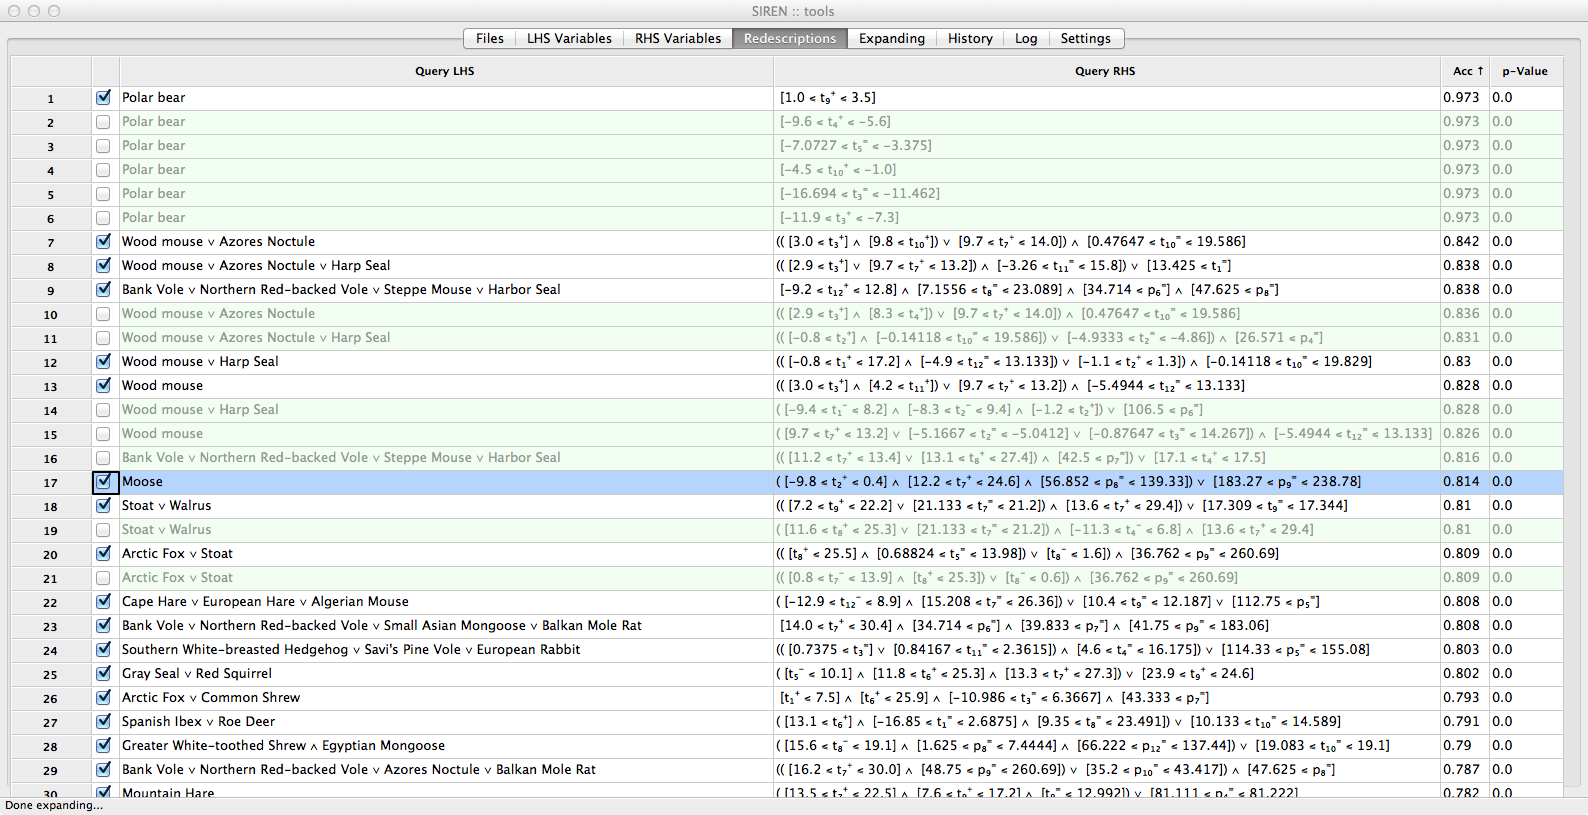
\includegraphics[width=.5\textwidth]{screenshots/redescriptions.png}
%   \caption{Tool panel, filtering redescriptions.}
%   \label{fig:filtering}
% \end{figure}

\prg{Outputting the results}
\label{sec:outputting-results}
Finally, \Siren\ facilitates the distribution of the results:
redescriptions can be exported in easy-to-read format and the
maps associated to redescriptions can be easily converted to
publication-ready files. 

\section{Applications}
We will demonstrate the application of \Siren\ on two application domains. 

\prg{Biological niche-finding}
An important problem in biology, known as \emph{niche-finding} is a
particular instance of redescription mining.  The bioclimatic
constraints that must be met for a certain species to survive
constitute that species' bioclimatic envelope, or niche~\cite{grinnell17niche}.  Finding such
envelopes can help, e.g.\ to predict the results of global
warming~\cite{pearson03predicting}.  A number of methods, involving
regression, neural networks, and genetic algorithms
(see~\cite{soberon05interpretation}) have been developped over the
past ten year to model the bioclimatic envelope.
\textsc{BIOMOD}~\cite{thuiller09biomod} being a good example of
a modelling tool used this domain.  But to the best of our
knowledge, none of these methods allows automatically finding both the
set of species and their envelope.

We demonstrate the application of \Siren\ on this task using a data
that describes spatial areas of Europe, squares of side roughly 50
km$^2$.  The left hand side data contains information about the
mammals that live in these areas, while the right hand side consists
of bioclimatic variables. The data comes from two publicly available
datasets: European mammal atlas~\cite{mitchell-jones99atlas} and
Worldclim climate data~\cite{hijmans05very}.

\prg{US counties statistics}

\begin{figure}
  \centering
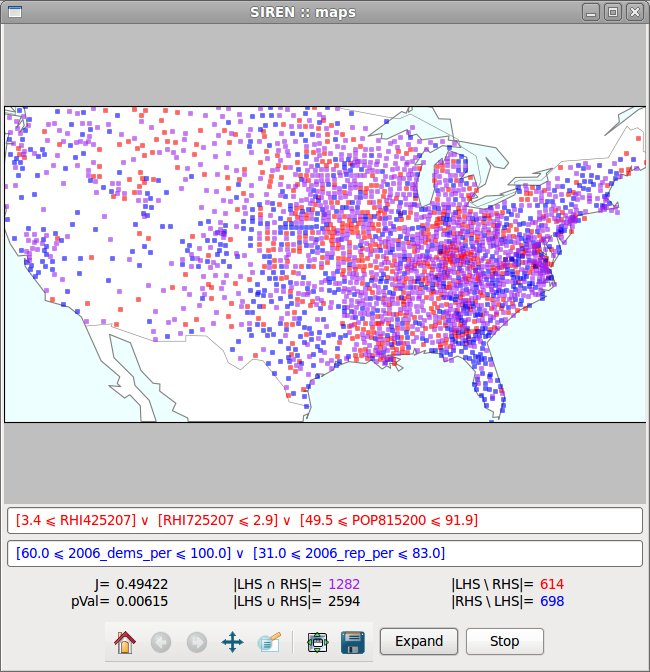
\includegraphics[width=.5\textwidth]{screenshots/siren_map_us_00.jpg}
  \caption{Map panel, displaying a redescription on a map.}
  \label{fig:map_panel}
\end{figure}


To demonstrate the flexibility of our tool, we illustrate its usage on a dataset from an entirely different domain, describing the counties of continental United-States. 
This time, the left hand side data contains socio-economic indicators about the counties, such as population, age distribution or educational attainment. The right hand side consists of data about funding of the electoral campaigns in 2006, 2008 and 2010. The data has been gathered from two public websites: FedStats\footnote{http://www.fedstats.gov/} and Open Secrets\footnote{http://www.opensecrets.org/elections/}.

\section{Implementation details}
\Siren\ as well as the back-end redescription mining algorithm \ReReMi, on which it relies, are implemented in Python.
The interface is built with the \texttt{wxPython} Open Source GUI toolkit, ensuring cross-platform compatibility.
The \texttt{matplotlib} library enables to generate high quality figures seamlessly integrated in the interface.
\Siren\ can handle any data provided in compatible format. 

\section{Related work}
\label{sec:related-work}
As opposed to data mining techniques like Emerging Patterns Mining
(EPM), Contrast Set Mining (CSM) or Subgroup Discovery (SD) (see
\cite{kralj09supervised} for a unifying survey), Redescription mining
aims at simultaneously finding multiple descriptions of a subset of
entities which is not previously specified, selecting the few relevant
among a potentially large set of variables. Since its introduction
in~\cite{ramakrishnan04turning} various algorithms have been proposed
for Boolean redescription mining, based on approaches including
decision trees~\cite{ramakrishnan04turning,kumar07redescription},
co-clusters~\cite{parida05redescription}, and frequent
itemsets~\cite{gallo08finding}.  

For its mining purposes, \Siren\
relies on the \ReReMi. This greedy algorithm extends redescription
mining to categorical and numerical variables using an efficient
on-the-fly discretization technique.

Currently, redescription mining is a purely descriptive approach, its
predictive power remains to be explored.

\section{Conclusions}
We present \Siren, a tool for interactively mining geospatial
redescriptions. It allows users to mine, vizualise, edit and extend
redescriptions.
We will give the chance to the public to experiment with \Siren\ and
together consider how this tool could be used to explore their own geospatial
data and help answer their data analysis need.

\bibliographystyle{abbrv}
%\nocite{*}
\bibliography{bibsiren}  

\balancecolumns
% That's all folks!
\end{document}

%%% Local Variables: 
%%% mode: latex
%%% TeX-master: t
%%% End: 
